%\documentclass[twocolumn,superscriptaddress,aps,prb,floatfix]{revtex4-1}
\documentclass[11pt]{article}
\usepackage{amsmath,graphicx}
%\usepackage[cmex10]{amsmath}
\usepackage{amssymb}
\usepackage{amsthm}
\usepackage{geometry}
\usepackage{graphicx}
\usepackage{epstopdf}
\usepackage{hyperref}
% \usepackage[francais]{babel}
\usepackage[applemac]{inputenc}
\usepackage{color}

%\usepackage{graphicx}% Include figure files
%\usepackage{dcolumn}% Align table columns on decimal point
%\usepackage{bm}% bold math
%\usepackage{color}
%\usepackage[caption=false]{subfig} 

\usepackage{listings}

\definecolor{dkgreen}{rgb}{0,0.6,0}
\definecolor{gray}{rgb}{0.5,0.5,0.5}
\definecolor{mauve}{rgb}{0.58,0,0.82}

\lstset{frame=tb,
  language=python,
  aboveskip=3mm,
  belowskip=3mm,
  showstringspaces=false,
  columns=flexible,
  basicstyle={\small\ttfamily},
  numbers=none,
  numberstyle=\tiny\color{gray},
  keywordstyle=\color{blue},
  commentstyle=\color{dkgreen},
  stringstyle=\color{mauve},
  breaklines=true,
  breakatwhitespace=true,
  tabsize=3
}

\newcommand {\lb} {{\langle}}
\newcommand {\rb} {{\rangle}}
\newcommand {\R} {{\mathbb{R}}}
\newcommand {\X} {{\tilde X}}
\newcommand {\w} {{\tilde w}}
\newcommand {\hh} {{k}}
\newcommand {\p} {{\tilde p}}
\newcommand {\RN} {{{\mathbb{R}}^N}}
\newcommand {\Z} {{\mathbb{Z}}}
\newcommand {\E} {{\mathbb{E}}}
\newcommand {\W} {{\cal{W}}}
\newcommand {\Fem} {F_{e}}
\newcommand {\For} {F_{o}}
\newcommand{\Exp}[1]{\mathbb{E}\left(#1 \right)}

\usepackage{amsthm}
\usepackage{amsmath}
\usepackage{amssymb}


\newcommand{\figref}[1]{Fig. \ref{#1}}


\newtheorem{theorem}{Theorem}[section]
\newtheorem{lemma}[theorem]{Lemma}
\newtheorem{proposition}[theorem]{Proposition}
\newtheorem{corollary}[theorem]{Corollary}

%\newenvironment{proof}[1][Proof]{\begin{trivlist}
%\item[\hskip \labelsep {\bfseries #1}]}{\end{trivlist}}
%\newenvironment{definition}[1][Definition]{\begin{trivlist}
%\item[\hskip \labelsep {\bfseries #1}]}{\end{trivlist}}
%\newenvironment{example}[1][Example]{\begin{trivlist}
%\item[\hskip \labelsep {\bfseries #1}]}{\end{trivlist}}
%\newenvironment{remark}[1][Remark]{\begin{trivlist}
%\item[\hskip \labelsep {\bfseries #1}]}{\end{trivlist}}

%\newcommand{\qed}{\nobreak \ifvmode \relax \else
%      \ifdim\lastskip<1.5em \hskip-\lastskip
%      \hskip1.5em plus0em minus0.5em \fi \nobreak
%      \vrule height0.75em width0.5em depth0.25em\fi}

\begin{document}

%\allowdisplaybreaks

\title{Topology and Geometry of Deep Rectified Network Optimization Landscapes}


%\author{C. Daniel Freeman \\ 
%daniel.freeman@berkeley.edu, Department of Physics, University of California, Berkeley, CA 94720, USA}

\author{C. Daniel Freeman and Joan Bruna \\
Department of Statistics, University of California, Berkeley, CA 94720, USA \\
Courant Institute of Mathematical Sciences, New York University, New York USA
}


\date{\today}

\maketitle

\begin{abstract}
The loss surface of deep neural networks has recently attracted interest 
in the optimization and machine learning communities as a prime example of 
high-dimensional non-convex problem. Some insights were recently gained using spin glass 
models, but at the expense of strongly simplifying the nonlinear nature of the model

In this work, we do not make any such assumption and prove that 
deep rectified networks do not have bad local minima. Together with 
recent results that rigorously establish that no gradient descent can 
get stock on saddle points, we conclude that gradient descent converges
to a global optimum in deep rectified networks.

The conditioning of such gradient descent is the next challenge we address. 
We study this question by estimating the geometry of level sets, and we introduce
an algorithm to estimate the regularity of such sets on large-scale networks. 
Our empirical results suggest that these sets become exponentially more curvy 
as the energy level decays, in accordance to what is observed in practice. 
 \end{abstract}

\tableofcontents

%%%%%%%%%%%%%%%%%%%%%%
%%%%%%%%%%%%%%%%%%%%%%
\section{Introduction}
\label{sec:Intro}
%%%%%%%%%%%%%%%%%%%%%%

\begin{itemize}
\item Context of the problem
\item Related work: Spin glass, recent result.
\item Gradient Descent converges to minimizers (Jordan Recht et al). 
\item Main result on connectedness of level sets.
\item Geometry of the level sets. Algorithm to estimate the geodesics along level sets. Measure of curvature of these sets. 
\end{itemize}
  


\section{Topology of Level Sets}

Let $P$ be a probability measure on a product space $\mathcal{X} \times \mathcal{Y}$, 
where we assume $\mathcal{X}$ and $\mathcal{Y}$ are Euclidean vector spaces for simplicity.
Let $\{ (x_i, y_i)\}_i$ be an iid sample of size $L$ drawn from $P$ defining the training set.
We consider the classic empirical risk minimization of the form
\begin{equation}
\label{emp_risk_min}
\Fem(\theta) = \frac{1}{L} \sum_{l=1}^L \| \Phi(x_i;\theta) - y_i \|^2~,
\end{equation}
where $\Phi(x ; \theta)$ encapsulates the feature representation 
that uses parameters $\theta \in \R^S$. In a deep neural network, this parameter
contains the weights and biases used in all layers.
For convenience, in our analysis we will also use the oracle risk minimization:
\begin{equation}
\label{risk_min}
\For(\theta) = \E_{(X,Y) \sim P} \| \Phi(X;\theta) - Y \|^2~,
\end{equation}

We define the level set of $F(\theta)$ as 
\begin{equation}
\Omega_F(\lambda) = \{ \theta \in \R^S~;~F(\theta) \leq \lambda \}~. 
\end{equation}

The first question we study is the structure of critical points of $\Fem(\theta)$ and $\For(\theta)$
when $\Phi$ is a multilayer neural network. In particular, we are interested to know whether
$\Fem$ has local minima which are not global minima. This question is answered by 
knowing whether $\Omega_F(\lambda)$ is connected at each energy level $\lambda$:

\begin{proposition}
If $\Omega_F(\lambda)$ is connected for all $\lambda$ then every local minima of $F(\theta)$ is a global minima. 
\end{proposition}
{\it Proof:} Suppose that $\theta_1$ is a local minima and $\theta_2$ is a global minima, 
but $F(\theta_1) > F(\theta_2)$. If $\lambda = F(\theta_1)$, then clearly 
$\theta_1$ and $\theta_2$ both belong to $\Omega_F(\lambda)$. Suppose 
now that $\Omega_F(\lambda)$ 
is connected. Then we could find a smooth (i.e. continuous and differentiable) path $\gamma(t)$ 
with $\gamma(0) = \theta_1$, $\gamma(1)= \theta_2$ and $F(\gamma(t)) \leq \lambda = F(\theta_1)$.
In particular, as $t \to 0$, we have
\begin{eqnarray*}
F(\gamma(t)) &=& F(\theta_1) + t \langle \nabla F(\theta_1) , \dot{\gamma}(0) \rangle + \frac{t^2}{2} \left(\dot{\gamma}(0)^T H F(\theta_1) \dot{\gamma}(0) + \langle \nabla F(\theta_1), \ddot{\gamma}(0) \rangle \right) + o(t^2) \\
&=& F(\theta_1) +   \frac{t^2}{2}  \dot{\gamma}(0)^T H F(\theta_1) \dot{\gamma}(0)  + o(t^2) ~,
\end{eqnarray*}
which shows that $F(\gamma(t)) \leq F(\theta_1)$ for all $t$ is incompatible with $H(\theta_1) \succeq 0$. $\square$


\subsection{The Linear Case}

A particularly simple but insightful case is 
when $F$ is a multilayer network defined by
\begin{equation}
\label{linearcase}
\Phi(x;\theta) = W_K \dots W_1 x~,~\theta = (W_1, \dots, W_K)~.
\end{equation}
This model defines a non-convex (and non-concave) loss $\Fem(\theta)$ 
which has been recently studied in \cite{linearcase} concurrently with our work. 
We provide here an alternative proof that in that case, there are no poor local 
minima.

%For that purpose, let $W_1, W_2, \dots, W_K$ be weight matrices of sizes 
%$n_k \times n_{k+1}$, $k < K$. Assume first that $n_j \geq \min(n_1, n_K)$ for $j=2 \dots K-1$.
%and let us define the following multilinear regression problem:
%\begin{equation}
%\label{multilinloss}
%L_0(W_1, \dots, W_K) = \sum_i \| W_K, \dots W_1 x_i - y_i \|^2~,
%\end{equation}
%where $\{ (x_i, y_i)\,; x_i \in \mathbb{R}^{n_1}, y_i \in \mathbb{R}^{n_K} \}_i$ is a given 
%training set. 

We have the following result.
\begin{proposition}
\label{proplinear}
Let $W_1, W_2, \dots, W_K$ be weight matrices of sizes 
$n_k \times n_{k+1}$, $k < K$, and let $\Fem(\theta)$, $\For(\theta)$ 
denote the risk minimizations using $\Phi$ as in (\ref{linearcase}).
Assume that $n_j \geq \min(n_1, n_K)$ for $j=2 \dots K-1$ [TODO I think this is not necessary].
Then $\Omega_{\Fem}(\lambda)$ is connected for all $\lambda$, as well as $\For$. 
\end{proposition}
{\it Proof:} We proceed by induction over the number of layers $K$. 
For $K=1$, the loss $F(\theta)$ is convex. Let  $\theta_1$, $\theta_2$ be two arbitrary points 
in a level set $\Omega_\lambda$. Thus $L(\theta_1) \leq \lambda$ and $L(\theta_2) \leq \lambda$. We have
$$L( t \theta_1 + (1-t) \theta_2) \leq t L(\theta_1) + (1-t) L(\theta_2) \leq \lambda~,$$
and thus a linear path is sufficient in that case to connect $\theta_1$ and $\theta_2$.

Suppose the result is true for $K-1$. Let $\theta_1 = (W_1^1, \dots, W^1_K)$ and 
 $\theta_2 = (W_1^2, \dots, W^2_K)$ with $L(\theta_1) \leq \lambda$, $L(\theta_2) \leq \lambda$.
For each $W_1, \dots, W_K$, we denote $\tilde{W}_j = W_j$ for $j < K-1$ and
$\tilde{W}_{K-1} = W_K W_{K-1}$. By induction hypothesis, the 
loss expressed in terms of $\tilde{\theta} = (\tilde{W}_1, \dots, \tilde{W}_{K-1})$ is connected 
between $\tilde{\theta}_1$ and $\tilde{\theta_2}$. Let $\tilde{W}_{K-1}(t)$ the corresponding 
path projected in the last layer. We just need to produce a path in the variables $W_{K-1}(t)$, $W_K(t)$ 
such that (i) $W_{K-1}(0) = W_{K-1}^1$, $W_{K-1}(1) = W_{K-1}^2$, 
(ii) $W_{K}(0) = W_{K}^1$, $W_{K}(1) = W_{K}^2$, and 
(iii) $W_{K}(t) W_{K-1}(t) = \tilde{W}_{K-1}(t)$ for $t \in (0,1)$. 
We construct it as follows. Let 
$$W_{K}(t) = t W_{K}^2 + (1-t) W_{K}^1 + t (1-t) V~,$$
$$W_{K-1}(t) = W_{K}(t)^\dagger \tilde{W}_{K-1}(t)  ~,$$
where $W_{K}(t)^\dagger = ( W_{K}(t)^T W_{K}(t))^{-1} W_{K}(t)^T$ denotes the pseudoinverse 
and $V$ is a $n_{K-1} \times n_{K}$ matrix drawn from a iid distribution. 
Conditions (i) and (ii) are immediate from the definition, and condition (iii) results from the fact that 
$$W_{K}(t) W_{K}(t)^\dagger  = {\bf I}_{N_K}~,$$
since $W_K(t)$ has full rank for all $t \in (0,1)$. 
$\square$.

\subsection{Half-Rectified Nonlinear Case}

We now study the setting given by 
\begin{equation}
\label{relucase}
\Phi(x;\theta) = W_K \rho W_{K-1} \rho \dots \rho W_1 x~,~\theta = (W_1, \dots, W_K)~,
\end{equation}
where $\rho(z) = \max(0 ,z)$. 
The biases can be implemented by replacing the input vector $x$ 
with $\overline{x}=(x, 1)$ and by rebranding each parameter matrix as 
$$\overline{W}_i = \left( 
\begin{array}{c|c}
W_i & b_i \\
\hline 
0 & 1 
\end{array}
\right)~,$$
where $b_i$ contains the biases for each layer.	
For simplicity, we continue to use $W_i$ and $x$ in the following.

We start with a characterization of the oracle loss. 
\begin{theorem}
Let $W_1, W_2, \dots, W_K$ be weight matrices of sizes 
$n_k \times n_{k+1}$, $k < K$, and let $\Fem(\theta)$, $\For(\theta)$ 
denote the risk minimizations using $\Phi$ as in (\ref{relucase}).
Assume that $n_j \geq \min(n_1, n_K)$ for $j=2 \dots K-1$ [TODO I think this is not necessary].
Then $\Omega_{\For}(\lambda)$ is connected for all $\lambda$. 
\end{theorem}
{\it Proof:}
We will again prove the result by induction over the depth $K$. 
Suppose first that $K=2$. The oracle risk is 
$$\For( W_1, W_2) = \Exp{ \| W_2 \rho W_1 X - Y \|^2}~.$$
If we denote $X_{W_1} = \rho W_1 X$, let us verify that $\For(W_1, W_2)$ 
only depends upon the correlation operator of $X_{W_1}$ 
and its cross-correlation to $Y$. Indeed, we have
\begin{eqnarray*}
\Exp{ \| W_2 \rho W_1 X - Y \|^2} &=& \Exp{ \| W_2 X_{W_1} - Y \|^2} \\
&=& W_2 \Sigma_{W_1} W_2^T + \Sigma_Y - 2  Tr\left( W_2 \Sigma_{W_1,Y} \right)~,
\end{eqnarray*}
where $\Sigma_{W_1} = \Exp{ X_{W_1} X_{W_1}^T}$ and $\Sigma_{W_1,Y} = \Exp{ X_{W_1} Y^T}$.
Let us see that when $\rho(z)$ is the half-rectification the covariance structure 
of $X_{W_1}$ can be easily related to the original distribution. Indeed, we have
the following
\begin{lemma}
Let $Z = \rho W X$ with $\rho(z) = \max(0,z)$. Then
\begin{equation}
\Sigma_Z = \tilde{W}^T \Sigma_X \tilde{W} 
\end{equation}
\end{lemma}

$\square$



[ TODO  $\Fem$ case]. 





%%%%%%%%%%%%%%%%%%%%%%
\section{Geometry of Level Sets}
%\section{Quantifying Nonconvexity}
\label{sec:QuanNoncon}

\subsection{Definitions}
\label{sec:Defs}
%%%%%%%%%%%%%%%%%%%%%%

 For a model with network parameters $\theta_i$, and a learning problem with sample space $X$, the fundamental object of study is the loss function, $L(X, \theta_i)$.  In practice, one only has access to an estimate of the loss function over some restricted subset, $\chi_i$, of the sample space: $E( L(X, \theta_i), \chi_i )$.  Unless otherwise stated, the loss functions computed throughout are assumed to be on a restricted test set not used during training.
 
 A key ingredient of the algorithm is the use of an \emph{interpolated model}.  For two given models, $\theta_1$ and $\theta_2$, we defined the interpolated model with parameter $t$ as follows:
 
\begin{equation}
\Theta (\theta_1 ,\theta_2, t) := \theta_1 (1-t) + \theta_2 t
\end{equation}

 Thus, the interpolated model parameters---i.e., weights and biases---are simply linearly interpolated between two given models.
 
 Additionally, the algorithm requires an estimate of the interpolated loss curve:

 \begin{equation}
 \gamma(\theta_1, \theta_2) := L (X ,\Theta (\theta_1, \theta_2, t)), t \in [0,1]
 \end{equation}

 or, an estimate of the loss on those models which are linear interpolations sitting between $\theta_1$ and $\theta_2$.  More specifically, we seek efficient estimates of the location of the maxima, $t^* := \frac{d \gamma(\theta_1, \theta_2, t)}{dt} \bigg|_{t^*} = 0, \frac{d^2 \gamma(\theta_1, \theta_2, t)}{dt^2} \bigg|_{t^*} < 0$.  While in principle, the interpolated loss curve could have rich structure, in practice it is generally fairly smooth, thus straightforward hill climbing algorithms can efficiently locate these points.
 
 Finally, for a pair of models $(\theta_1, \theta_2)$, it will be convenient to define the maximum interpolated error:
 
  \begin{equation}
  \Gamma(\theta_1, \theta_2) := \rm{min}_{\Theta^*(\theta_1, \theta_2)}\:\rm{max}\:L (X, \theta_i) \bigg|_{\theta_i \in \Theta^*} \label{eq:minmaxerror}
  \end{equation}
 
 where $\Theta^* (\theta_1, \theta_2)$ is \emph{any} continuous path in the space of weights connecting $\theta_1$ and $\theta_2$.  Thus, $\Gamma(\theta_1, \theta_2)$ represents the minimum possible maximum loss achieved by those paths in the space of weights connecting $\theta_1$ and $\theta_2$.  More intuitively, if $\Gamma (\theta_1, \theta_2) \leq \rm{max}\: (L(X,\theta_1), L(X,\theta_2))$, then the models are ``connected''---there exists a continuous path in the space of models with total loss never exceeding the maximum loss achieved by $\theta_1$ or $\theta_2$. 
 
 \subsection{The Greedy Algorithm}
 \label{sec:GreedyAlg}
 
 1. Train two models $\theta_i$ and $\theta_j$ to a threshold loss value, $L_0$.
 
 2. Determine the location of the global maxima, $t^*$, on the interpolated loss curve $\gamma(\theta_i, \theta_j)$. 
 
 3. Perform gradient descent on the interpolated model $\Theta (\theta_i, \theta_j, t^*) := \theta_{i,j}$ until it is below $\alpha L_0$ for some $\alpha \in [0,1]$ .
 
 4. Calculate the maxima of the interpolated losses $\gamma(\theta_i, \theta_{i,j})$ and $\gamma(\theta_{i,j}, \theta_j)$.  If these maxima are below $L_0$, then stop recursing on this branch and proceed to remaining branches(see 5).  If not, proceed to step 5.
 
 5. For those pairs, $\theta_a, \theta_b$ from step 4 for which the maxima exceeds $L_0$, start a new branch by returning to step 2 and making the replacement $i->a$ and $j->b$.  If depth exceeds $d$, stop (see below).
 
 \begin{figure}
\begin{center}
\scalebox{1}{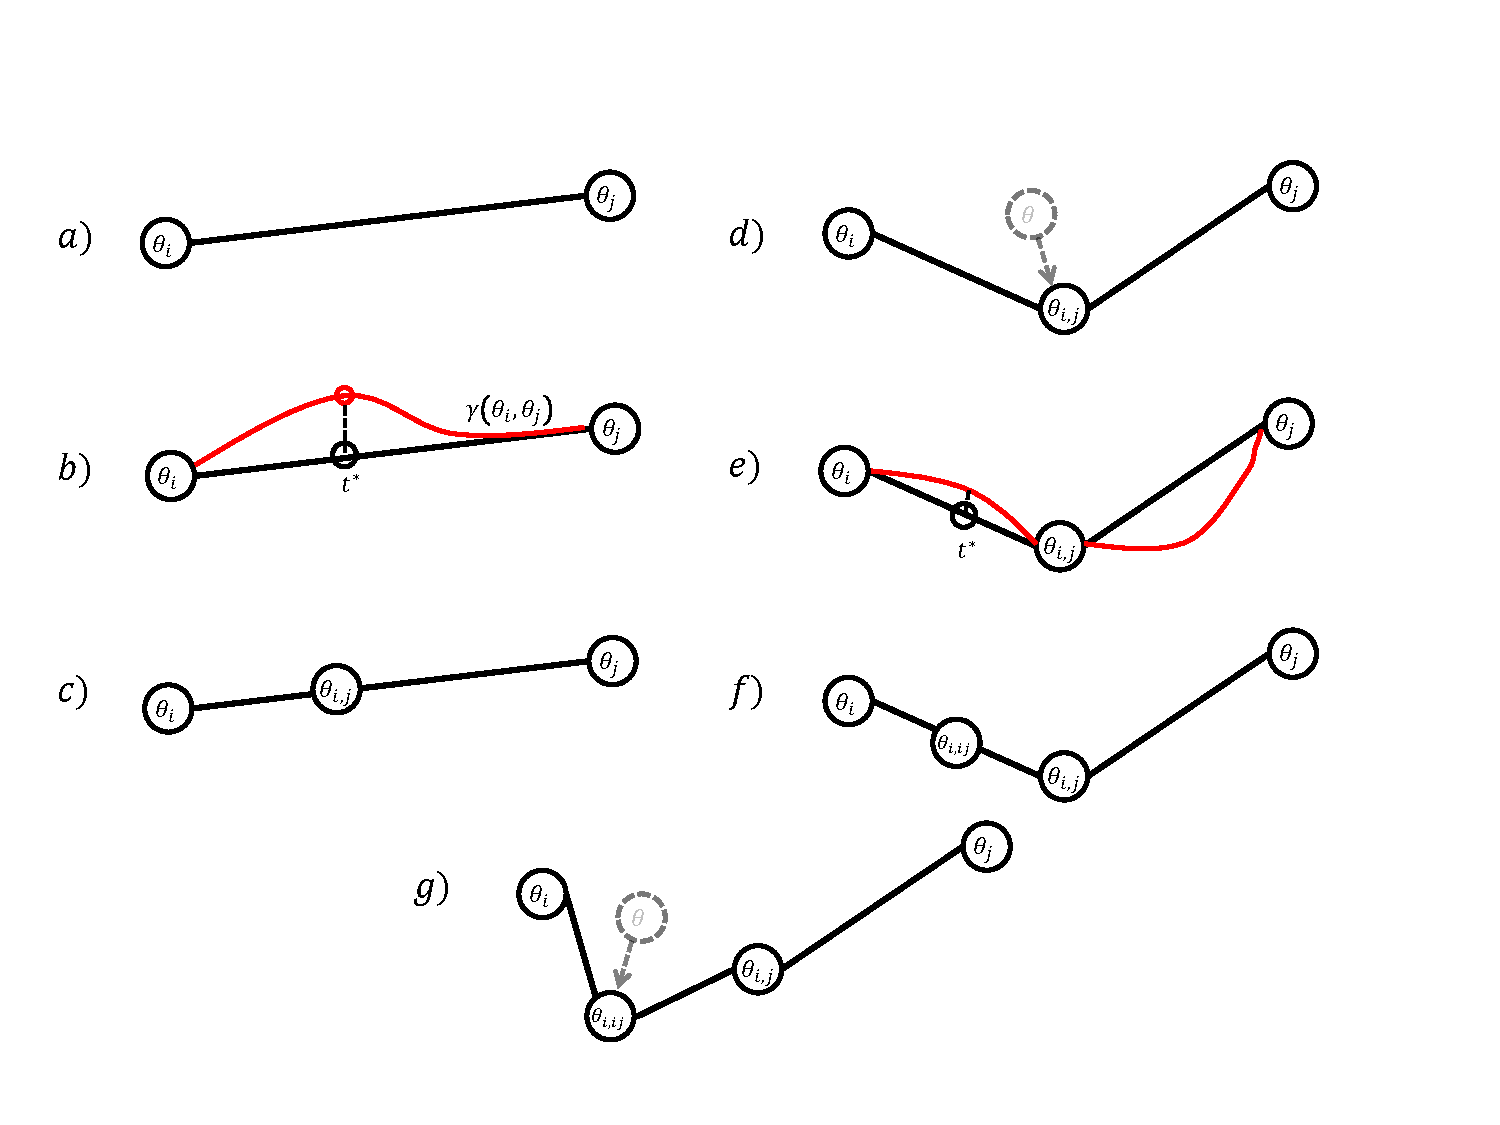
\includegraphics[width=1.0\columnwidth]{AlgorithmFigure}}
\end{center}
\caption{A cartoon of the algorithm.  $a):$ The initial two models with approximately the same loss, $L_0$. $b):$ The interpolated loss curve, in red, and its global maximum, occuring at $t=t^*$. $c):$ The interpolated model $\Theta(\theta_i, \theta_j, t^*)$ is added and labeled $\theta_{i,j}$.  $d):$ Stochastic gradient descent is performed on the interpolated model until its loss is below $\alpha L_0$. $e):$ New interpolated loss curves are calculated between the models, pairwise on a chain.  $f):$ As in step $c)$, a new model is inserted at the maxima of the interpolated loss curve between $\theta_i$ and $\theta_{i,j}$.  $g):$  As in step $d)$, gradient descent is performed until the model has low enough loss.}
\label{fig:AlgorithmFigure}
\end{figure}
 
 We provide a cartoon of the algorithm in \figref{fig:AlgorithmFigure}.  If the algorithm succeeds, then the output of the algorithm is a sequence of models, $\theta_i$ such that the pairwise interpolated loss curve between each in a sequence will be less than the threshold $L_0$.  Thus, the algorithm outputs a continuous path in parameter space connecting the original two models such that everywhere along the path, the total loss is less than or equal to the loss of the original models.
 
 As written, if a path does \emph{not} exist, then the algorithm will clearly not converge.  Thus, on top of the parameter $\alpha$, discussed below, the algorithm has an additional free parameter in the \emph{depth} chosen to explore.  For convenience, we define the string of models produced by the algorithm at depth $d$ with parameter $\alpha$ to be the \emph{interpolated string}, $S(\theta_1, \theta_2, \alpha, d)$.  These are precisely those models recursively generated by the algorithm in step 3.  Further, these models are naturally ordered along a path, starting from $\theta_1$ and terminating on $\theta_2$, as indicated in \figref{fig:AlgorithmFigure}.
 
 Finally, to use this as a tool to diagnose convexity, we define the \emph{maximum interpolated error at depth $d$ and tolerance $\alpha$}:
 
 \begin{align}
 \tilde{\Gamma}( \theta_1, \theta_2, d, \alpha ) &:= \rm{max}\ \gamma(\theta_i, \theta_j, t)\\ \notag
 &i,\ j\ \rm{neighbors\ in}\ S(\theta_1, \theta_2, \alpha, d)
 \end{align}
 
 where by ``neighbors in $S(\theta_1, \theta_2, \alpha, d)$'', we only mean that the models are immediately adjacent on the interpolating string.  This quantity upper bounds the true maximum interpolated error, i.e. \eqref{eq:minmaxerror}.
 
 In summary: the algorithm recursively produces and trains new models lying on a continuous path in the space of model parameters, i.e. a string.  Training via gradient descent biases the path towards valleys on the loss surface, thus encouraging the loss along this path to be low.  In practice, the parameter $\alpha$ is chosen to be less than 1 to aid convergence.  We provide numerical and theoretical evidence for this choice in section SECTIONGOHERE.
 

  \subsection{Constrained Dynamic String Sampling}
  \label{sec:ConstrainedAlg}
  
  While the algorithm presented in Sec. \ref{sec:GreedyAlg} is fast for sufficiently smooth families of loss surfaces with few saddle points, here we present a slightly modified version which, while slower, provides more control over the convergence of the string.  Instead of training intermediate models via full SGD to a desired accuracy, intermediate models will be subject to a constraint that ensures they are ``close'' to the neighboring models on the string.  Specifically, intermediate models will be constrained to the unique hyperplane in weightspace equidistant from its two neighbors.  This is similar to a sort of ``$L_1$ regularization'' where the loss function for a given model on the string, $\theta_i$, has an additional term $\tilde{L}(\theta) = L(\theta)+\zeta(\|\theta_{i-1} - \theta_i\|+\|\theta_{i+1} + \theta_i\|)$.  The strength of the $\zeta$ regularization term controls the ``springy-ness'' of the weightstring. note: make this more precise, the hyperplane constraint is stronger than the $L_1$ constraint...$L_1$ only keeps the model in a ball close to the midpoint between the models.
  
  Because adapting DSS to use this constraint is straightforward, here we will describe an alternative ``breadth-first'' approach wherein models are trained in parallel until convergence.  This alternative approach has the advantage that it will indicate a disconnection between two models ``sooner'' insofar as it will be clear two models cannot be connected once the loss on either of the two initial models, $\theta_1$ or $\theta_2$, is less than $\Gamma(\theta_1, \theta_2)$.  The precise geometry of the loss surface will dictate which approach to use in practice.
  
  Given two random models $\sigma_i$ and $\sigma_j$ where $|\sigma_i - \sigma_j| < \kappa$, we aim to follow the evolution of the family of models connecting $\sigma_i$ to $\sigma_j$.  Intuitively, almost every continuous path in the space of random models connecting $\sigma_i$ to $\sigma_j$ has, on average, the same (high) loss.  For simplicity, we choose to initialize the string to the linear segment interpolating between these two models.  If this entire segment is evolved via gradient descent, the segment will either evolve into a string which is entirely contained in a basin of the loss surface, or some number of points will become fixed at a higher loss.  These fixed points are difficult to detect directly, but will be indirectly detected by the persistence of a large interpolated loss between two adjacent models on the string.
  
  The algorithm proceeds as follows:
  
  (0.) Initialize model string to have two models, $\sigma_i$ and $\sigma_j$.
  
  1. Begin training all models to the desired loss, keeping the instantaneous loss of all models being trained approximately constant..
  
  2. If the pairwise interpolated loss $\gamma(\sigma_n,\sigma_{n+1})$ exceeds a tolerance $\alpha_1$, insert a new model at the maximum of the interpolated loss between these two models.  For simplicity, this tolerance is chosen to be $(1 + \alpha_1^*)$ times the instantaneous loss of all other models on the string.  
  
  3. Repeat steps (1) and (2) until all models (and interpolated errors) are below a threshold loss $L_0$, or until a chosen failure condition (see \ref{sec:Fail}).
  
  \subsection{Failure Conditions}
  \label{sec:Fail}
  
  While the algorithms presented will faithfully certify two models are connected if the algorithm converges, it is worth reemphasizing that they do not guarantee that two models are disconnected if the algorithm fails to converge.  In general, the problem of determining if two models are connected can be made arbitrarily difficult by choice of a particularly pathological geometry for the loss function, so we are constrained to heuristic arguments for determining when to stop running the algorithm.
  
  Thankfully, in practice, loss function geometries for problems of interest are not intractably difficult to explore.
 

 
 %%%%%%%%%%%%%%%%%%%%%%
\section{Numerical Experiments}
\label{sec:NumExp}

For our numerical experiments, we aimed to extract qualitative features of both small, toy networks, as well as of larger workhorse networks suitable for use on real world tasks (e.g. MNIST).  At its core, the maximum interpolated error (i.e., \eqref{eq:minmaxerror}) is a measure of problem nonconvexity---or, more precisely, of the nonconvexity of the loss surface of a given architecture on a particular learning problem.


\subsection{Polynomial Regression}
\label{sec:PolyFuncs}
%%%%%%%%%%%%%%%%%%%%%%

 Polynomial function regression is a task for which small neural networks can achieve extremely high accuracy.  For our numerical experiments, we studied a 1-4-4-1 fully connected multilayer perceptron style architecture with RELU activation and RMSProp optimization.  For ease-of-analysis, we restricted the family of polynomials to be strictly contained in the interval $x\in[0,1]$ and $f(x)\in[0,1]$.
 
 Discussion of different Loss functions
 
 etc.


%%%%%%%%%%%%%%%%%%%%%%
\subsection{Convolutional Neural Networks}
\label{sec:CNN}
%%%%%%%%%%%%%%%%%%%%%%



%%%%%%%%%%%%%%%%%%%%%%
%%%%%%%%%%%%%%%%%%%%%%
\section{Discussion}
\label{sec:Discussion}
%%%%%%%%%%%%%%%%%%%%%%
\begin{itemize}
\item Future: Generalization Error Question. 

\end{itemize}
 
 

\bibliography{nonconvex}

\end{document}
%
% {**}{**}{**} End of file apssamp.tex {**}{**}{**}
